\documentclass[a4paper,10pt]{article}
\usepackage{graphicx}
\usepackage{verbatim}
\usepackage{subfig}
\usepackage{float}
\usepackage[spanish]{babel}   %ver bien como es
\usepackage[utf8]{inputenc}
\usepackage{tabularx}
\hyphenation{des-com-po-ner-los va-rie-dad in-gre-dien-tes ac-tua-li-za-cio-nes me-dian-te con-si-de-ra-cio-nes nues-tro au-to-ma-ti-za-do pro-pues-tos con-tras-ta-das ra-zo-na-ble}

\begin{document}

\tableofcontents

\newpage


\section*{Introducci\'on}
\addcontentsline{toc}{section}{Introducci\'on}


\newpage
\section*{Presunciones}
\addcontentsline{toc}{section}{Presunciones}


\newpage


\section*{Vistas}
\addcontentsline{toc}{section}{Vistas}
En esta secci\'on presentaremos las diferentes especificaciones realizadas durante el presenta trabajo pr\'actico.
Se explicar\'a como se abord\'o cada parte del trabajo, explicando para que momentos fue utilizada cada t\'ecnica de especificaci\'on, y el porque
de esta desici\'on.

En un aspecto general, se divieron las t\'ecnicas de especificaci\'on seg\'un los siguientes crit\'erios:

\begin{itemize}
\item Modelo Conceptual: Se utilizar\'a para un entendimiento global del funcionamiento del sofware, entiendendo las entidas que interactuan dentro y con el mismo.
\item Diagrama de Casos de Uso: Se utilizar\'a para mostrar todas las interacciones que la m\'aquina tiene con los diversos actores.
\item Diagramas de Actividad: Se utilizar\'an para mostrar secuencias de acciones, usualmente agruparan diversos casos de uso que posean un hilo conductor.
\item Maquinas de Estado Finitas: Se utilizar\'an para mostrar las acciones que ocurren principalmente dentro de la m\'aquina para de esta manera, junto a los dem\'as esqumas
, poder dar un panorama completo del comportamiento del software.
\end{itemize}


\bigskip

\subsection*{Modelo Conceptual}
\addcontentsline{toc}{subsection}{Modelo Conceptual}

\subsection*{Diagrama de Casos de Uso}
\addcontentsline{toc}{subsection}{Diagrama de Casos de Uso}

Esta t\'ecnica sirve para mostrar como son las interacciones entre el mundo y la m\'aquina, es decir que se abstraen varias de las relaciones presentes
obviando las relaciones prop\'ias entre actores que se encuentran por fuera de la m\'aquina, as\'i como las interacciones que son intr\'insecas de la m\'aquina.

\subsubsection*{Diagrama}
\addcontentsline{toc}{subsubsection}{Diagrama}

A continuaci\'on se presenta el diagrama de casos de uso para toda la m\'aquina, es decir, se engloban todas las interacciones en un mismo diagrama
y luego se detallar\'a en particular cada caso de uso.


\begin{figure}[H]
\centering
\subfloat{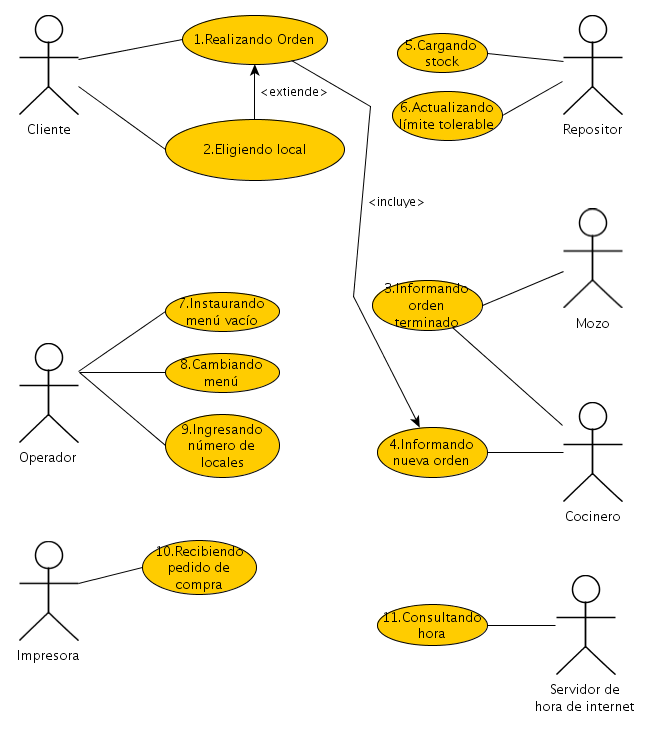
\includegraphics[width=1.3\textwidth]{Imagenes/CasosDeUso.png}}
\caption{Diagrama de Casos de Uso}
\end{figure}


\subsubsection*{Detalles Casos de Uso}
\addcontentsline{toc}{subsubsection}{Detalles de Casos de Uso}

A continuaci\'on se detallar\'a cada caso de uso, dando la descripci\'on de la sucesi\'on de hechos, adem\'as de los actores y la pre y postcondici\'on.

Para seguir un hilo conductor, los casos de uso se encuentran numerados en forma secuencial agrupados por el o los actores participantes.

Se seguir\'a este mismo secuenciamiento para realizar la descripci\'on.

\bigskip


En primer lugar se encuentra unos de los casos de uso m\'as importante en todo el funcionamiento de la pizzer\'ia. La realizaci\'on de un nuevo
pedido por parte del cliente.


\begin{center}
\begin{tabularx}{14cm}{|X|X|}
\hline
\multicolumn{2}{|l|}{Nombre Casos de uso: Realizando orden}\\
\hline
\multicolumn{2}{|l|}{Actores: Cliente}\\
\hline
\multicolumn{2}{|l|}{Precondici\'on: True}\\
\hline
\multicolumn{2}{|l|}{PostCondici\'on: Se logra hacer el pedido}\\
\hline
Curso Normal & Curso Alternativo\\
\hline
1.1 El cliente realiza una orden. & 1.2 La orden no es válida. Fin de C.U.
\\
\hline
2.1 El sistema verifica que se puede realizar la orden (si hay stock). &
\\
\hline
3.1 En caso de que haya stock, el sistema toma el pedido. &
\\
\hline
3.1.1 Se incluye el caso de uso ``Informando nueva orden''. &
\\
\hline
4.1 En caso de que no haya stock, el sistema notifica que no se puede realizar el pedido. &
\\
\hline
4.1.1 Se extiende al caso de uso ``Eligiendo local''. &
\\
\hline
5.1 Fin del C.U. & \\
\hline
\end{tabularx}
\end{center}


\bigskip

\begin{center}
\begin{tabularx}{14cm}{|X|X|}
\hline
\multicolumn{2}{|l|}{Nombre Casos de uso: Eligiendo Local}\\
\hline
\multicolumn{2}{|l|}{Actores: Cliente}\\
\hline
\multicolumn{2}{|l|}{Precondici\'on: El cliente realiz\'o un pedido que no se puede efectuar en el propio local}\\
\hline
\multicolumn{2}{|l|}{PostCondici\'on: El cliente elige un nuevo local}\\
\hline
Curso Normal & Curso Alternativo\\
\hline
1.1 El cliente recibe una lista de locales donde se puede satisfacer su pedido & 
\\
\hline
2.1 El cliente elige un local de la lista recibida & 2.2 El cliente no eligen ning\'ung local. Ir a 4.1.
\\
\hline
3.1 El software debe informar la nueva orden en el local elegido. Se incluye Caso de Uso Informando Nueva Orden &
\\
\hline
4.1 Fin Caso de Uso &
\\
\hline
\end{tabularx}
\end{center}

Este caso de uso, en contraste a la mayor\'ia de los dem\'as, contiene una precondici\'on. Este se incluye para imponer una restricci\'on que no
se puede imponer desde el diagrama mismo dado a que no existe expresividad para esto. 

La precondici\'on del caso de uso dice El cliente realiz\'o un pedido que no se puede efectuar en el propio local.
Esta precondici\'on se incluye para mostrar que este caso de uso no tiene sentido por si solo sin una precedencia directa del caso de uso
Realizando Nueva Orden. Esto no se puede expresar en el diagrama mismo dado que la etiqueta presente en la relaci\'on entre los dos casos de uso 
aparece la etiqueta extiende. Esto es as\'i dado que no siempre que se realiza una nueva orden se elige otro local, por lo que no ser\'ia correcta
la inclusi\'on de una etiqueta incluye. Luego, se usa esta precondici\'on para indicar esta restricci\'on y para poder la descripci\'on del caso de uso
ya asumiendo que el cliente realiz\'o una orden que no pudo ser satisfecha en el propio local.

\bigskip

\begin{center}
\begin{tabularx}{14cm}{|X|X|}
\hline
\multicolumn{2}{|l|}{Nombre Casos de uso: Informando Orden Terminada}\\
\hline
\multicolumn{2}{|l|}{Actores: Mozo, Cocinero}\\
\hline
\multicolumn{2}{|l|}{Precondici\'on: Existe una orden en proceso}\\
\hline
\multicolumn{2}{|l|}{PostCondici\'on: Se informa que hay se finaliz\'o una orden}\\
\hline
Curso Normal & Curso Alternativo\\
\hline
1.1 El cocinero cocina una pizza que se encontraba en una orden en proceso & 
\\
\hline
2.1 El cocinero ingresa en el sistema la finalizaci\'on de la orden pertinente & 
\\
\hline
3.1 El software actualiza el sistema de ordenes, tildando como realizada la orden que el cocinero notific\'o &
\\
\hline
4.1 El software avisa al mozo correspondiente que la orden se encuentra finalizada para retirar &
\\
\hline
5.1 El mozo se entera que se termin\'o una orden y queda dispuesto a ir a buscar la orden para su entrega &
\\
\hline
\end{tabularx}
\end{center}

\bigskip

\begin{center}
\begin{tabularx}{14cm}{|X|X|}
\hline
\multicolumn{2}{|l|}{Nombre Casos de uso: Eligiendo Local}\\
\hline
\multicolumn{2}{|l|}{Actores: Cliente}\\
\hline
\multicolumn{2}{|l|}{Precondici\'on: El cliente realiz\'o un pedido que no se puede efectuar en el propio local}\\
\hline
\multicolumn{2}{|l|}{PostCondici\'on: El cliente elige un nuevo local}\\
\hline
Curso Normal & Curso Alternativo\\
\hline
1.1 El cliente recibe una lista de locales donde se puede satisfacer su pedido & 
\\
\hline
2.1 El cliente elige un local de la lista recibida & 2.2 El cliente no eligen ning\'ung local. Ir a 4.1.
\\
\hline
3.1 El software debe informar la nueva orden en el local elegido. Se incluye Caso de Uso Informando Nueva Orden &
\\
\hline
4.1 Fin Caso de Uso &
\\
\hline
\end{tabularx}
\end{center}






\subsection*{Diagramas de Actividad}
\addcontentsline{toc}{subsection}{Diagrmas de Actividad}

\subsection*{M\'aquinas de Estado Finita}
\addcontentsline{toc}{subsection}{M\'aquinas de Estado Finita}


\newpage


\section*{Discusi\'on}
\addcontentsline{toc}{section}{Discusi\'on}




\newpage
\section*{Conclusiones}
\addcontentsline{toc}{section}{Conclusiones}





\end{document}
